\ifdefined\pdfoutput\pdfoutput=1\fi
\documentclass[11pt]{article}
\usepackage[final]{acl}
\usepackage{times}
\usepackage{latexsym}
\usepackage[T1]{fontenc}
\usepackage[utf8]{inputenc}
\usepackage{microtype}
\usepackage{amsmath,amssymb,booktabs,graphicx,tabularx}
\usepackage{enumitem}

\title{Multidimensional Continuous Scoring of Chinese Metaphor Texts}
\author{Anonymous ACL submission}

\begin{document}
\raggedbottom
\maketitle
\begin{abstract}
Metaphor texts vary in familiarity, imageability, and the extent to which they convey figurative meaning. Assigning scores to these properties supports the selection and comparison of materials for language research. We study multidimensional continuous scoring of Chinese metaphor texts, predicting mean human ratings within a specified interval. Our approach draws on automated essay scoring: a model evaluates text against explicit criteria, while human-rated examples connect those criteria to a numerical scale. We adapt this scoring approach to metaphor-related properties and introduce Calibrated Ensemble for Metaphor Scoring (CEMS), which combines a rubric-guided large language model with ratings of semantically similar examples and regression from text embeddings. The combination is fitted separately for each dimension using training data. We evaluate the framework on two Chinese rating datasets, with comparisons to individual predictors and task-adapted scoring methods. The evaluation examines numerical error, item ranking, and the contribution of each source of scores.
\end{abstract}

\section{Introduction}

Metaphor texts differ in how familiar, meaningful, and easy to imagine they are, as well as in how strongly they convey figurative meaning. Researchers use ratings of these properties to select materials and compare experimental conditions. Chinese metaphor datasets record such judgments as mean human ratings on defined scales \citep{huang2024cogmed,wang2022normed}. As new materials are introduced, researchers need scores on the same dimensions. This motivates multidimensional continuous scoring: given an expression and a rating dimension, predict its mean human rating within the specified interval.

\begin{figure*}[t!]
\centering
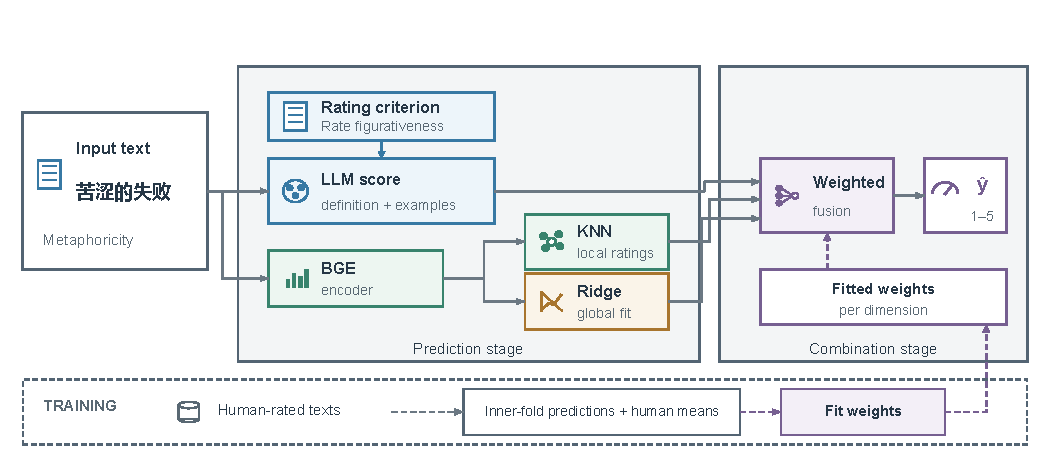
\includegraphics[width=\textwidth]{figures/fig_cems_architecture.pdf}
\caption{CEMS predicts one rating dimension for an input expression. The LLM uses the dimension criterion and rated examples; frozen BGE embeddings feed a nearest-neighbor predictor and a Ridge regressor. The combiner applies dimension-specific weights and an intercept. Dashed arrows show training: inner-fold predictions are paired with human means to fit the combiner.}
\label{fig:cems}
\end{figure*}

Automated essay scoring (AES) offers a relevant starting point. AES assigns numerical scores to texts according to assessment criteria, including separate scores for different writing traits \citep{do2024arts,eltanbouly2025trates}. Metaphor scoring shares this need to connect a judgment about text to a bounded numerical scale. Individual essay grades may be discrete, while the mean human ratings predicted here are continuous. The methodological connection is the use of explicit criteria and human-scored examples to guide numerical prediction. It allows us to draw on text-scoring methods developed in education when designing a scorer for metaphor-related properties.

In particular, rubric-based approaches make the dimensions of assessment explicit. TRATES uses trait-specific rubric questions to derive features for essay scoring \citep{eltanbouly2025trates}. AutoSCORE, developed for scoring student responses, separates the extraction of rubric-relevant components from the assignment of a score \citep{wang2026autoscore}. These methods concern educational assessment; they were not proposed for metaphor scoring. We borrow the principle of evaluating text against stated criteria, and adapt the criteria and prediction target to human judgments of metaphor texts.

This adaptation requires more than replacing an essay with a shorter expression. Essay rubrics assess aspects of student performance, whereas metaphor rating dimensions describe properties of an expression. A familiar expression need not be highly figurative, and a high score on one property does not imply a high score on another. Each predicted score must correspond to the definition of its dimension. It must also place that judgment on the scale used by human raters: a description such as ``familiar'' does not by itself specify a numerical mean. Existing human-rated expressions provide examples of how the definitions are used and where texts fall on the scale.

Our question is how to combine judgments guided by dimension definitions with the numerical information in existing human ratings. The definitions specify what to assess; rated texts show how people use the scale. We study this combination for continuous prediction across metaphor-related dimensions. We introduce CEMS, which connects an LLM's interpretation of each rating definition with predictions learned from rated examples. The LLM receives the definition, a rating question, and examples from the training set. A nearest-neighbor predictor estimates the score from semantically similar rated expressions, while an embedding regression model learns text--score relationships across the training set. Their scores are combined using weights fitted separately for each dimension, allowing the contributions of the predictors to vary with the rated property.

We evaluate CEMS on COGMED and Wang's Chinese sentence ratings. The experiments compare its numerical predictions with human means, examine item rankings, and test the contribution of each predictor. We also implement task-specific adaptations of AutoSCORE and RULERS-guided direct scoring, a rubric-based approach to general text evaluation \citep{hong2026rulers}. These comparisons examine how different scoring procedures carry over to metaphor ratings. 

Our contributions are:
\begin{itemize}[leftmargin=*,nosep]
    \item We develop an AES-inspired approach to multidimensional continuous scoring of Chinese metaphor texts, with metaphor-related rating definitions and mean human scores as the prediction target.
    \item We introduce CEMS, which combines criterion-guided LLM scores with predictions from semantically similar rated expressions and embedding regression, using dimension-specific weights learned from training data.
    \item We evaluate continuous scoring on two Chinese datasets through comparisons with individual predictors and adapted scoring frameworks, component ablations, and analyses of item ranking.
\end{itemize}



\section{Related Work}

\subsection{Automated essay and student-response scoring}

AES predicts human-assigned scores for student essays, either as an overall grade or as separate trait scores. ArTS generates multiple trait scores autoregressively \citep{do2024arts}. TRATES uses trait-specific rubrics to generate assessment questions, then combines the resulting features with other essay features in a regression model \citep{eltanbouly2025trates}. These approaches connect dimension-specific assessment with numerical prediction.

AutoSCORE addresses automated scoring in educational assessment \citep{wang2026autoscore}. An extraction agent identifies rubric-relevant components in a student response, and a scoring agent uses the structured representation to assign scores. Its original inputs, rubrics, and evaluation concern student work. Our AutoSCORE-adapted baseline replaces them with metaphor expressions, metaphor rating definitions, and rated examples from the target dataset. The resulting comparison evaluates this adaptation to metaphor scoring. CEMS draws on the broader criterion-guided scoring approach, with a single LLM scoring branch and two predictors learned from human ratings.

\subsection{Rubric-based text evaluation}

Rubric-based scoring also appears in the evaluation of generated text. G-Eval uses LLMs to evaluate text under specified criteria \citep{liu-etal-2023-g}. LLM-Rubric combines rubric-question response distributions in a calibration network to predict human judgments across dimensions \citep{hashemi2024llmrubric}. CEMS instead combines a continuous LLM score with two text-based rating predictors, using a separate constrained combination for each dimension. RULERS uses a fixed rubric, evidence-supported judgments, and score calibration \citep{hong2026rulers}. These are general text-evaluation approaches, distinct from AES and metaphor rating. We use a local adaptation of RULERS-guided direct scoring as a comparison; its score calculation and the omitted calibration stage are specified in Section~\ref{sec:adaptations}.

\subsection{Human ratings of metaphor texts}

Metaphor rating datasets describe properties such as familiarity, meaningfulness, and imageability \citep{huang2024cogmed,wang2022normed}. These ratings characterize expressions rather than student performance. Recent work examines how closely LLM judgments reproduce human metaphor ratings and how they handle source--target mappings \citep{mangiaterra2025gptnorms,pissani2026llmnorms,zhou2026tastingemotions}. Work on English and Chinese semantic norms also compares prompted LLMs with predictors trained on text embeddings \citep{peng2025multilingualnorms}. We combine the two prediction routes in one scorer: a definition-guided LLM judgment and estimates learned directly from rated text embeddings. Our framework uses a dimension's definition to guide the LLM and human-rated examples to learn numerical predictions for new items from the same task.

\section{Task Definition}

We treat metaphor rating as a multidimensional regression task. Each dimension describes a property of the text and has a bounded rating scale. The target is the mean of human judgments, which can take fractional values even when individual raters select discrete scale points. Scores describe the property specified by each dimension, rather than a general measure of text quality.

Let $\mathcal{D}=\{(x_i,\mathbf{y}_i)\}_{i=1}^{N}$ be a dataset in which $x_i$ is a Chinese expression and $\mathbf{y}_i=(y_{i1},\ldots,y_{iK})$ gives its mean human ratings on $K$ dimensions. We have ratings for a training subset $\mathcal{D}_{\mathrm{tr}}$ and want to predict $\hat{\mathbf{y}}_i$ for unscored items in $\mathcal{D}_{\mathrm{te}}$. Training and test items come from the same rating task. Predictions use only $\mathcal{D}_{\mathrm{tr}}$, the item text, and the definitions of the rating dimensions.

We predict the mean human rating for each item, rather than an individual participant's response. Evaluation uses grouped five-fold cross-validation. In COGMED, normalized duplicate expressions stay in the same group. In Wang, sentence variants from the same item family stay together. Thus, each test fold contains unseen item families, with training examples drawn from the same task.

Each dataset supplies its own labeled training set and fitted predictors. The evaluation measures prediction for new texts under the same rating definitions. Our Wang scorer uses the three corresponding COGMED definitions in its prompts and is fitted to the reconstructed Wang ratings. This evaluates prediction within each task.
\section{Method}

CEMS adapts criterion-guided text scoring to the continuous rating task defined above. Here, a rubric consists of a metaphor-related dimension definition and a corresponding rating question. The LLM uses these criteria and rated examples to assign a score. Two additional predictors estimate human ratings from semantic neighbors and text embeddings. The LLM and BGE encoder remain frozen in the main configuration. Human ratings supply prompt examples and KNN neighbor labels, train the Ridge regressor, and determine the fusion weights and intercept.

Figure~\ref{fig:cems} shows how we fit the fusion weights on training data and use them to predict ratings for test items.



\subsection{Rubric-guided LLM score}

For each item and dimension, Qwen3-14B-AWQ receives the expression, the dimension definition, a rating question, and five examples retrieved from the training set and rated on that dimension. It returns a continuous score on a working scale of $[1,5]$. Retrieved examples exclude the target item and its group. Fusion uses the score; confidence and free-form rationales are not input features.

The LLM also proposes a source--target mapping and quotes evidence from the expression or available context. A validator checks whether each quote matches the stated source span. This check verifies the location of the quoted text. We test a version without the mapping prompt in an ablation.

\subsection{Semantic predictors}

We encode each expression with the frozen BAAI/bge-small-zh-v1.5 encoder \citep{xiao2024cpack}. For each dimension, BGE-KNN averages the human ratings of the five nearest training items, weighted by similarity. BGE-Ridge uses regularized linear regression to predict human means from normalized embeddings. Both use labels from the current training fold. 

\subsection{Fitting the fusion weights}

Let $\mathbf{p}_{id}=(q_{id},k_{id},r_{id})$ denote the LLM, KNN, and Ridge scores for item $i$ and dimension $d$. We learn dimension-specific nonnegative weights $\mathbf{w}_d$ that sum to one and an intercept $\beta_d$:
\begin{equation}
\hat{y}_{id}=\operatorname{clip}_{[1,5]}
\left(\mathbf{w}_d^\top\mathbf{p}_{id}+\beta_d\right).
\label{eq:fusion}
\end{equation}
We select weights using predictions generated by four-fold cross-validation within the outer training set. Each inner fold is held out in turn: prompt examples and KNN neighbors come from the remaining inner folds, and Ridge is fitted on those folds. The frozen LLM and encoder are reused throughout. Pooling the held-out predictions gives one out-of-fold (OOF) score from each branch for every outer-training item. We compare combinations of these scores against the corresponding human means using MAE. For each weight vector on the 0.05 simplex grid, we set the intercept to the median training residual, clipped to $[-0.5,0.5]$, and evaluate the resulting clipped predictions. We select the candidate with the lowest OOF MAE. We then refit the semantic predictors on the full outer training set and use the fixed fusion parameters on the test fold. Human labels in the outer test fold are never used for retrieval, regression, or calibration.

\section{Experimental Setup}

\subsection{Datasets}

\paragraph{COGMED.} COGMED contains 671 Chinese metaphors related to smell and taste, with human mean ratings on seven dimensions: familiarity, meaningfulness, metaphoricity, valence, difficulty, imageability, and naturalness \citep{huang2024cogmed}. We predict the original means. For difficulty, the prompt asks the LLM to predict the released numerical rating using labeled examples to infer its direction. We retain the original values without reversal; the evaluation measures agreement with this field, whose endpoint meanings were not established in our source extraction.

\paragraph{Wang.} Wang's materials contain 120 families, each with a novel metaphor, a simile, a literal sentence, and an anomalous sentence \citep{wang2022normed}. We use the first three classes, giving 360 candidate items. Strict text matching across the material list and public participant-rating sheets yields 356 items with all three rating dimensions. Our targets are arithmetic means reconstructed from the exported familiarity, meaningfulness, and metaphoricity ratings. Appendix~\ref{sec:wang_data} describes aggregation and exclusions. We reuse the definitions of these three dimensions from COGMED. During fitting, Wang's scores are linearly mapped from the original 1--7 scale to $[1,5]$; predictions are mapped back for evaluation. Sentence variants share a family identifier and stay together in each split.

\subsection{Models, baselines, and validation}

We use Qwen3-14B-AWQ as the primary scoring model \citep{yang2025qwen3}. We also test Qwen3-8B on both tasks and Llama-3.1-8B-Instruct on COGMED. BGE stays frozen in the semantic branches. The rubric-guided LLM tests scoring from dimension definitions and rated examples. BGE-KNN and BGE-Ridge test prediction directly from human-rated texts, without an LLM scoring step. The LLM with an intercept fitted on OOF predictions tests whether correcting an overall score offset is sufficient. We compare these baselines with CEMS on the same outer splits and with access to the same training labels.

We use five-fold grouped cross-validation, training on four folds and testing on the remaining fold. Within each outer training set, four inner folds produce OOF predictions for fitting fusion weights. The Wang extension uses the additional selection and calibration steps in Appendix~\ref{sec:appendix_extension}. All reported metrics use outer-test predictions.

\subsection{Adapted scoring baselines}
\label{sec:adaptations}

On COGMED, AutoSCORE-adapted tests an extraction--scoring procedure transferred from educational assessment, while RULERS-adapted tests direct scoring under a fixed rubric adapted from general text evaluation. Both use the same frozen Qwen3-14B-AWQ model, temperature 0, seven dimension definitions, five retrieved training examples, and grouped outer folds. These adaptations request all seven dimensions together; CEMS requests each dimension separately. The comparisons therefore include differences in output format as well as scoring procedure.

\paragraph{AutoSCORE-adapted.} AutoSCORE was developed for scoring student responses in educational assessment \citep{wang2026autoscore}. We replace its educational rubrics and student responses with metaphor rating definitions and expressions, retaining the extraction--scoring design. The first agent extracts dimension-relevant observations, quotations, and uncertainties. A separate scoring agent receives these components, the expression, dimension definitions, and rated examples, and returns continuous human-mean predictions on $[1,5]$.

\paragraph{RULERS-adapted (direct score).} Inspired by the locked-rubric execution stage of \citet{hong2026rulers}, we compile one task-level rubric with three checklist items and five scale anchors per dimension. The judge receives this rubric, the expression, and rated examples, and returns a continuous \texttt{score} for each dimension alongside checklist decisions and evidence fields. We evaluate the direct score on $[1,5]$, without rounding or reconstructing it from checklist decisions. This adaptation omits the original RULERS calibration stage. Both adapted baselines are evaluated before post-processing, whereas CEMS includes a fitted score combination. This comparison evaluates the complete implemented pipelines, with output organization and calibration as part of their differences.  Appendix~\ref{sec:adapter_details} provides implementation and evaluation details.

\subsection{Metrics}

Mean absolute error (MAE) is the primary metric because the task is to estimate continuous human mean scores. Root mean squared error (RMSE) gives greater weight to large errors. Pearson correlation measures linear association, and Spearman correlation measures agreement in item ranking. Quadratic weighted kappa (QWK) provides an auxiliary measure of agreement after discretization. Metrics are computed separately for each dimension and then averaged equally across dimensions. Error and correlation metrics use the task's original score scale. QWK rounds both human means and predictions to the nearest integer on the original scale. We report 95\% confidence intervals for paired MAE differences using bootstrap resampling of the outer-test predictions. Appendix~\ref{sec:bootstrap_details} specifies the resampling units and settings.

\section{Results}

\subsection{Overall continuous scoring performance}

CEMS gives the lowest MAE and RMSE among the compared systems on both datasets (Tables~\ref{tab:cogmed} and~\ref{tab:wang}). On COGMED, macro MAE decreases from 0.292 for the rubric-guided LLM to 0.265 for CEMS. The paired difference is $-0.0270$ (95\% CI $[-0.0350,-0.0198]$). On Wang, MAE decreases from 0.602 to 0.549 on the original 1--7 scale. The corresponding intercept-only baselines obtain 0.289 and 0.564. Thus, combining the predictors improves the estimates of human means beyond correcting an overall score offset.

\begin{table*}[t]
\centering
\small
\setlength{\tabcolsep}{7pt}
\caption{Macro-averaged COGMED results over seven dimensions. The LLM receives five rated examples. Adapted scoring pipelines use the same backbone and training-example pool; RULERS-adapted uses the judge's direct continuous score (Section~\ref{sec:adaptations}).}
\label{tab:cogmed}
\begin{tabular}{lrrrrr}
\toprule
Method & MAE $\downarrow$ & RMSE $\downarrow$ & Pearson $\uparrow$ & Spearman $\uparrow$ & QWK $\uparrow$\\
\midrule
BGE-KNN & 0.304 & 0.409 & 0.670 & 0.633 & 0.471\\
BGE-Ridge & 0.380 & 0.473 & 0.618 & 0.597 & 0.183\\
Rubric-guided LLM & 0.292 & 0.411 & 0.715 & 0.700 & 0.544\\
LLM + intercept calibration & 0.289 & 0.406 & 0.715 & 0.699 & \textbf{0.579}\\
CEMS & \textbf{0.265} & \textbf{0.361} & \textbf{0.750} & \textbf{0.721} & 0.537\\
\midrule
\multicolumn{6}{l}{\textit{Adapted scoring pipelines (Section~\ref{sec:adaptations})}}\\
AutoSCORE-adapted & 0.311 & 0.446 & 0.676 & 0.665 & 0.511\\
RULERS-adapted (direct score) & 0.336 & 0.480 & 0.638 & 0.629 & 0.498\\
\bottomrule
\end{tabular}
\end{table*}
\begin{table*}[t]
\centering
\small
\setlength{\tabcolsep}{7pt}
\caption{Macro-averaged Wang results on the original 1--7 scale.}
\label{tab:wang}
\begin{tabular}{lrrrrr}
\toprule
Method & MAE $\downarrow$ & RMSE $\downarrow$ & Pearson $\uparrow$ & Spearman $\uparrow$ & QWK $\uparrow$\\
\midrule
BGE-KNN & 0.970 & 1.253 & 0.537 & 0.436 & 0.459\\
BGE-Ridge & 1.147 & 1.332 & 0.563 & 0.475 & 0.212\\
Rubric-guided LLM & 0.602 & 0.810 & \textbf{0.829} & \textbf{0.750} & 0.793\\
LLM + intercept calibration & 0.564 & 0.772 & 0.827 & 0.744 & \textbf{0.804}\\
CEMS & \textbf{0.549} & \textbf{0.745} & 0.827 & 0.736 & 0.796\\
\bottomrule
\end{tabular}
\end{table*}






\paragraph{Adapted scoring frameworks.}
\label{sec:adapter_results}
On the same 671 COGMED test items, AutoSCORE-adapted obtains MAE 0.3113, compared with 0.2652 for CEMS. The paired difference is $+0.0461$ (95\% group-bootstrap CI $[0.0333,0.0597]$). CEMS also has lower RMSE and higher correlations and QWK. RULERS-adapted direct scoring obtains MAE 0.3361 on the same items. Its paired MAE difference from CEMS is $+0.0709$ (95\% group-bootstrap CI $[0.0580,0.0850]$). Thus, CEMS estimates human means more closely than either adapted pipeline under the specified evaluation conditions.

\subsection{Performance across rating dimensions}

CEMS lowers MAE on all seven COGMED dimensions (Table~\ref{tab:dimension_mae}). The largest absolute reductions are in naturalness, from 0.353 to 0.292, and metaphoricity, from 0.357 to 0.312. Familiarity changes less, from 0.389 to 0.376, and remains the dimension with the highest error. The improvements therefore extend across the rated properties, with different magnitudes. These dimension-level point estimates show where the overall gain occurs; the component ablations below examine which predictors contribute to it.

\begin{table}[t]
\centering
\small
\setlength{\tabcolsep}{5pt}
\caption{COGMED MAE by dimension for the rubric-guided LLM and CEMS.}
\label{tab:dimension_mae}
\begin{tabular}{lrr}
\toprule
Dimension & LLM & CEMS\\
\midrule
Familiarity & 0.389 & 0.376\\
Meaningfulness & 0.249 & 0.234\\
Metaphoricity & 0.357 & 0.312\\
Valence & 0.227 & 0.209\\
Difficulty & 0.213 & 0.200\\
Imageability & 0.258 & 0.233\\
Naturalness & 0.353 & 0.292\\
\bottomrule
\end{tabular}
\end{table}

\subsection{Contribution of the scoring components}

The COGMED ablation in Table~\ref{tab:ablation} removes each component and refits the remaining fusion weights. Removing the LLM raises MAE by 0.0345 (95\% CI $[0.0255,0.0434]$), the largest increase. Removing BGE-KNN raises MAE by 0.0076 ($[0.0037,0.0115]$), showing that ratings from semantic neighbors add information to the remaining predictors. Removing the intercept raises MAE by 0.0043 ($[0.0015,0.0074]$).

The change after removing BGE-Ridge is only 0.0010, with an interval spanning zero; its removal also increases QWK from 0.537 to 0.565. The ablation primarily supports combining the LLM with semantic-neighbor ratings. Evidence for an additional contribution from Ridge is weaker.

\begin{table}[t]
\centering
\small
\caption{COGMED component ablation. $\Delta$MAE is the ablated model minus full fusion; intervals use paired item bootstrap.}
\label{tab:ablation}
\begin{tabular}{lrr}
\toprule
Configuration & $\Delta$MAE & 95\% CI\\
\midrule
Remove LLM & 0.0345 & [0.0255, 0.0434]\\
Remove BGE-KNN & 0.0076 & [0.0037, 0.0115]\\
Remove BGE-Ridge & 0.0010 & [-0.0006, 0.0027]\\
Remove intercept & 0.0043 & [0.0015, 0.0074]\\
\bottomrule
\end{tabular}
\end{table}

\paragraph{Mapping prompt.}
On COGMED, MAE is 0.292 with explicit mapping extraction and 0.296 without it. The paired MAE difference is $-0.0039$ (95\% CI $[-0.0120,0.0040]$), providing no clear evidence of an accuracy gain from explicit mapping extraction.

\subsection{Performance with different scoring models}

Fusion lowers MAE in all five model--task combinations in Appendix Figure~\ref{fig:backbones}: by 9.2\%, 8.7\%, and 43.7\% for the three COGMED models, and by 8.9\% and 11.6\% for the two Wang models. The direction of improvement is consistent across these point estimates. Llama's larger relative gain reflects its higher initial error; it does not indicate better final scores than the Qwen models. Appendix Table~\ref{tab:backbone_all} reports the absolute scores and all auxiliary metrics.



\subsection{Score accuracy and item ranking}

The auxiliary metrics distinguish accuracy in score values from agreement in item ordering. On COGMED, CEMS has the highest Pearson and Spearman correlations among the compared systems. On Wang, both correlations are slightly lower than for the uncalibrated LLM, despite lower MAE. For agreement after rounding, intercept-only calibration has the highest QWK on both datasets: 0.579 versus 0.537 for CEMS on COGMED, and 0.804 versus 0.796 on Wang. Improving continuous predictions does not guarantee the same ordering or rounded score assignments.

Wang also permits a closer examination within sentence classes. Given the class label, a training-set class-median predictor obtains MAE 0.4718, compared with 0.5485 for text-only CEMS. This diagnostic uses additional metadata and indicates that class differences are informative about score levels. Within novel metaphors, CEMS has Spearman correlation 0.062. An exploratory representation and calibration variant reaches 0.190, still a weak association (Appendix~\ref{sec:appendix_extension}). The pooled results therefore need to be read alongside within-class results when the intended use is to rank similar metaphor materials.

\section{Discussion}

\paragraph{Adapting criterion-guided scoring.}
The connection with AES lies in evaluating text against explicit criteria and relating those judgments to human scores. For metaphor texts, the criteria describe properties such as familiarity and metaphoricity, each with its own interpretation. CEMS implements this connection through dimension-specific prompts and rated examples. The contribution is the combination of these judgments with predictions learned from human-rated texts. The component comparisons identify the sources of predictive gains within this design.

\paragraph{Using human-rated examples.}
Rated expressions serve two roles: they illustrate the scale in the LLM prompt and provide labels for numerical predictors. The improvement over intercept-only correction, together with the KNN ablation, supports using semantic-neighbor ratings alongside the LLM's judgment. The weaker Ridge contribution shows that adding another supervised predictor does not necessarily provide useful additional information. These findings concern new items drawn from the same rating task as the training examples.

\paragraph{Interpreting continuous scores.}
The dimension-level analysis shows that errors vary across the properties being rated. A single average score across dimensions conceals this variation. The lower MAE supports estimating approximate rating levels. Selecting between closely matched expressions also requires useful within-class ranking. The weak novel-metaphor correlations on Wang identify a concrete boundary for that use. Human judgments remain important when small differences between candidate materials determine their selection.

\paragraph{Evidence and score validity.}
The mapping prompt provides an interpretation and quotations that can be checked against the text. Validating a quotation establishes its location, not the correctness of the mapping or its role in producing the score. Evidence traceability and numerical agreement with human ratings therefore require separate evaluation.

\section{Conclusion}

We predict human mean ratings for new Chinese metaphor items using rated examples from the same task. Combining a rubric-guided LLM with semantic neighbors and embedding regression lowers macro MAE on two datasets under grouped cross-validation and in all five tested model--task combinations. On COGMED, it also gives lower MAE than the local AutoSCORE and RULERS-guided direct-score adaptations. Component ablations identify the LLM and semantic-neighbor ratings as the main contributors on COGMED. The framework supports prediction of continuous rating levels, while the Wang analysis distinguishes this use from ranking closely matched texts within a sentence class.

\newpage
\section*{Limitations}

Both tasks use labels from the same task. Repeated dataset analysis during development is not captured by bootstrap intervals over saved predictions. The targets are mean ratings, which do not describe individual differences.

\section*{Ethical Considerations}

We use existing norm datasets and collect no new participant data. The outputs describe aggregate judgments about texts and should not be interpreted as assessments of individual participants.

\bibliography{references}

\clearpage
\appendix
\makeatletter
\setlength{\@fptop}{0pt}
\setlength{\@fpsep}{16pt}
\setlength{\@dblfptop}{0pt}
\setlength{\@dblfpsep}{16pt}
\makeatother
\section{Implementation and Supplementary Results}

\subsection{Wang data preparation}
\label{sec:wang_data}

We reconstruct item means from the public participant-rating exports. For each dimension, we average finite numerical responses in the original 1--7 range, excluding 11 invalid familiarity cells and one invalid metaphoricity cell. Text matching uses Unicode normalization and whitespace removal. We retain items with ratings on all three dimensions and omit four whose texts differ between the material list and the rating headers: families 44 and 93 (familiarity), 98 (metaphoricity), and 104 (meaningfulness). The retained set contains 119 novel metaphors, 119 similes, and 118 literal sentences across 120 families. Our targets are these reconstructed export means; equivalence to the original study's final norms, including its participant exclusion procedure, has not been established.

\subsection{Implementation details}

The rubric-guided LLM uses temperature 0 and returns one continuous score per requested dimension. Each request includes the original expression, a dimension definition, a rating question, and five same-dimension labeled examples retrieved by character TF--IDF cosine similarity. The scorer output is constrained to $[1,5]$ and is parsed as JSON. The evidence prompt returns source and target domains, a mapping relation, and quotations with source positions. Quotations are checked against the original input.

BGE embeddings are 512-dimensional normalized vectors. BGE-KNN uses $k=5$ with neighbor weights $\max(\cos(\mathbf{z}_i,\mathbf{z}_j),0.01)$. BGE-Ridge uses $\alpha=10$. Fusion weights lie on a 0.05 grid, are nonnegative, and sum to one; for each weight vector, the intercept is the median OOF residual clipped to $[-0.5,0.5]$. Candidates are selected by MAE, with ties broken by RMSE and then distance to equal weights. The outer-training predictions used to select fusion weights are generated by four inner folds. After selection, semantic predictors are refitted on the complete outer-training portion.

COGMED contributes 671 final outer-test predictions and 2,684 inner OOF predictions per scorer. Wang contributes 356 and 1,424, respectively. The inner OOF records are used for fitting and are not counted as test observations. Model inference used a single RTX 4090. Prompts, run configurations, item IDs, and training-side prediction records are archived with the project.

\subsection{Implementation of the adapted baselines}
\label{sec:adapter_details}

The COGMED comparison evaluates AutoSCORE-adapted and RULERS-adapted on the same 671 outer-test items as CEMS. Item identifiers, human ratings, and outer folds are matched across methods.

For each item--fold combination, retrieved examples exclude the outer test fold, the item's original fold, its own ID, and its family. For a test item, examples can come from the other four folds. The shared rubric is compiled from task definitions without human labels. AutoSCORE-adapted passes extracted components to its scoring agent. RULERS-adapted uses the judge's continuous \texttt{score} field on $[1,5]$; checklist decisions and confidence are auxiliary outputs and are not converted into the reported score. Outputs are parsed as JSON with a score for every rating dimension.

\subsection{Statistical comparisons}
\label{sec:bootstrap_details}

Paired percentile bootstrap intervals use 2,000 replicates. The COGMED component and mapping analyses resample items; the Wang analyses resample the 120 item families. The COGMED adapted-baseline comparisons resample groups with seed 20261029, pairing predictions by item and outer fold. The COGMED analysis set contains 671 groups of one item each, so item and group resampling use the same sampling units. These comparisons use the adapted methods' direct continuous scores and the saved CEMS predictions. No multiple-comparison correction is applied.

\subsection{Backbone results}

\begin{figure*}[t]
\centering
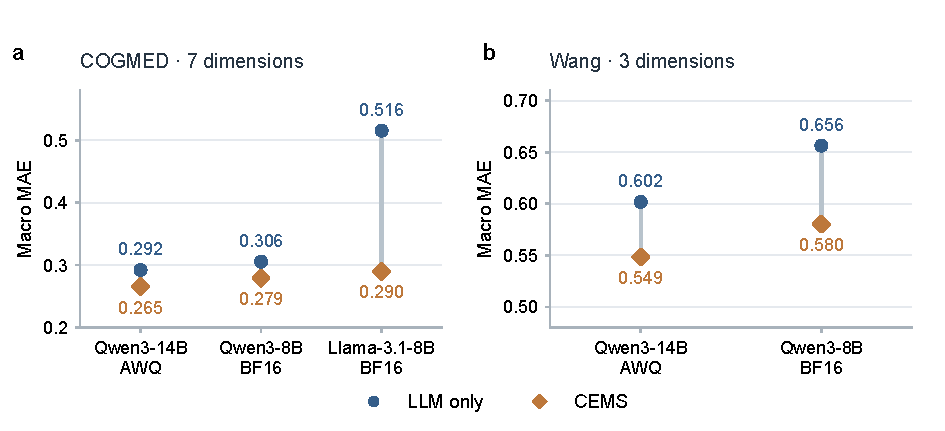
\includegraphics[width=0.88\textwidth]{figures/backbone_comparison.pdf}
\caption{Macro MAE for rubric-guided LLM scores and CEMS across five scorer--task pairs. The two panels use different original rating scales.}
\label{fig:backbones}
\end{figure*}

Table~\ref{tab:backbone_all} reports all five metrics for the five scorer--task pairs. The fusion MAE is lower in every pair. Other metrics vary by task and backbone.

\begin{table*}[t]
\centering
\footnotesize
\setlength{\tabcolsep}{5pt}
\caption{Full macro-averaged results for scorer--task pairs.}
\label{tab:backbone_all}
\begin{tabular}{lllrrrrr}
\toprule
Task & Scorer & Method & MAE & RMSE & Pearson & Spearman & QWK\\
\midrule
COGMED & Qwen3-14B-AWQ & LLM & 0.292 & 0.411 & 0.715 & 0.700 & 0.544\\
COGMED & Qwen3-14B-AWQ & CEMS & 0.265 & 0.361 & 0.750 & 0.721 & 0.537\\
COGMED & Qwen3-8B & LLM & 0.306 & 0.429 & 0.665 & 0.639 & 0.483\\
COGMED & Qwen3-8B & CEMS & 0.279 & 0.381 & 0.713 & 0.681 & 0.484\\
COGMED & Llama-3.1-8B & LLM & 0.516 & 0.721 & 0.493 & 0.516 & 0.374\\
COGMED & Llama-3.1-8B & CEMS & 0.290 & 0.393 & 0.693 & 0.658 & 0.448\\
Wang & Qwen3-14B-AWQ & LLM & 0.602 & 0.810 & 0.829 & 0.750 & 0.793\\
Wang & Qwen3-14B-AWQ & CEMS & 0.549 & 0.745 & 0.827 & 0.736 & 0.796\\
Wang & Qwen3-8B & LLM & 0.656 & 0.867 & 0.813 & 0.745 & 0.745\\
Wang & Qwen3-8B & CEMS & 0.580 & 0.760 & 0.815 & 0.739 & 0.759\\
\bottomrule
\end{tabular}
\end{table*}

\subsection{Wang extension protocol}
\label{sec:appendix_extension}

This exploratory variant replaces BGE-Ridge with a kernel regressor using frozen Qwen3-8B embeddings and applies half-strength isotonic calibration. MAE falls from 0.5485 to 0.5149. The differences from single-LLM isotonic calibration ($-0.0145$, 95\% CI $[-0.0301,0.0012]$) and the supervised-BGE extension ($-0.0109$, $[-0.0248,0.0038]$) have intervals that include zero. The following protocol specifies the representation selection and calibration steps.


The exploratory experiment uses six frozen Qwen3-8B representations: the final-token vector, last-layer mean pooling, and last-four-layer mean pooling, each for the original expression and an expression with a task prefix. Each has 4,096 dimensions. The search includes these six representations and BGE, a linear kernel and RBF kernels with $\gamma\in\{2,8\}$, and regularization values $\{0.001,0.01,0.1,1,10,100\}$, giving $7\times3\times6=126$ settings. We calculate candidate errors on four inner training folds, then refit the selected representation and kernel on the full outer training set.

For each outer fold and dimension, we select the representation, fit fusion weights, and fit isotonic calibration using outer-training labels. Inner predictions from the selected candidate are used to fit the fusion weights. Fusion scores for the outer-training items are then used to fit the monotone calibration map. Outer-test labels are used only for evaluation. The outer test fold stays independent, but the training predictions used for fusion and calibration are not produced by a fully nested cross-fitting procedure.

The supervised-BGE control fine-tunes the encoder with a LayerNorm and three-output linear head. It uses AdamW, learning rates $2\times10^{-5}$ for the encoder and 0.002 for the head, batch size 16, SmoothL1 loss with $\beta=0.3$, and candidate training epochs $\{2,5,10,20\}$ selected within outer training.

\begin{table*}[t]
\centering
\footnotesize
\setlength{\tabcolsep}{5pt}
\caption{Selected Wang representation and calibration comparisons on the original 1--7 scale.}
\label{tab:wang_all_exploration}
\begin{tabular}{lrrrrr}
\toprule
Configuration & MAE & RMSE & Pearson & Spearman & QWK\\
\midrule
CEMS & 0.549 & 0.745 & 0.827 & 0.736 & 0.796\\
Single LLM + isotonic & 0.529 & 0.720 & 0.834 & 0.732 & 0.791\\
Base fusion + isotonic & 0.533 & 0.731 & 0.833 & 0.722 & 0.794\\
Fixed-feature three-way fusion & 0.532 & 0.705 & 0.844 & \textbf{0.765} & 0.810\\
Fixed-feature fusion + half isotonic & \textbf{0.515} & \textbf{0.684} & \textbf{0.848} & 0.759 & \textbf{0.813}\\
Supervised BGE three-way fusion & 0.542 & 0.728 & 0.832 & 0.747 & 0.803\\
Supervised BGE fusion + half isotonic & 0.526 & 0.706 & 0.838 & 0.744 & 0.801\\
\bottomrule
\end{tabular}
\end{table*}


\subsection{Sentence-class analysis}

Table~\ref{tab:class_prior} compares text-only prediction with predictors that use known sentence classes. Table~\ref{tab:within_class} then examines rankings within each class.

\begin{table*}[t]
\centering
\footnotesize
\setlength{\tabcolsep}{5pt}
\caption{Wang class-information diagnostic. The class-based predictors receive sentence-type metadata unavailable to text-only CEMS.}
\label{tab:class_prior}
\begin{tabular}{lrrrrr}
\toprule
Predictor & MAE & RMSE & Pearson & Spearman & QWK\\
\midrule
CEMS (text only) & 0.549 & 0.745 & 0.827 & 0.736 & 0.796\\
Known class: training mean & 0.478 & 0.622 & 0.858 & 0.706 & 0.803\\
Known class: training median & 0.472 & 0.628 & 0.857 & 0.704 & 0.815\\
Known class: baseline + residual & 0.466 & 0.619 & 0.863 & 0.756 & 0.821\\
\bottomrule
\end{tabular}
\end{table*}


Table~\ref{tab:within_class} reports metrics separately within each sentence type for the base model and the fixed-feature fusion with half-strength isotonic calibration.

\begin{table*}[t]
\centering
\footnotesize
\setlength{\tabcolsep}{3pt}
\caption{Wang within-class metrics for the base model and the exploratory extension.}
\label{tab:within_class}
\begin{tabular}{llrrr}
\toprule
Class & System & MAE & Pearson & Spearman\\
\midrule
Literal & CEMS & 0.526 & 0.136 & 0.149\\
Literal & Extension & 0.482 & 0.180 & 0.208\\
Novel met. & CEMS & 0.596 & 0.063 & 0.062\\
Novel met. & Extension & 0.549 & 0.197 & 0.190\\
Simile & CEMS & 0.524 & 0.166 & 0.188\\
Simile & Extension & 0.514 & 0.215 & 0.234\\
\bottomrule
\end{tabular}
\end{table*}

\end{document}
